\subsection{Implementatie Datamodel}
Het ontwerp dat is gemaakt, mist een specifieke implementatie voor het gegevenstype \qw{content}, zoals te zien is in figuur \ref{fig:ClassDiagramItemFieldWithDefinition} (raadpleeg sectie \ref{subsection:Datamodel} voor meer details).
Dit gegevenstype zou verschillende vormen van gegevens moeten kunnen bevatten, zoals strings, getallen en booleans.
In programmeertalen zoals Python en Javascript is dit geen probleem, omdat ze dynamisch getypeerd zijn.
Dit betekent dat het gegevenstype van variabelen niet van tevoren gespecificeerd hoeft te worden.
Een van de randvoorwaarden is dat het afstudeerproduct gerealiseerd wordt in C\# wat een statisch getypeerde taal.
% Echter, het afstudeerproject moet worden gerealiseerd in een statisch getypeerde taal (C\#).

\whitespace
Dit is opgelost door gebruik te maken van een abstracte baseclass \textit{FieldValueBase}.
Deze baseclass  heeft verschillende implementaties die de verschillende datatypes kunnen ondersteunen.
Een klassendiagram hiervan is te zien in figuur \ref{fig:ImplementatieFields}.
In het klassendiagram is er één implementatie getoond van \textit{FieldValueBase} om het voorbeeld simpel te houden.

\whitespace
\begin{graphic}
    \captionsetup{type=figure}
    \caption{Implementaite Fields}
    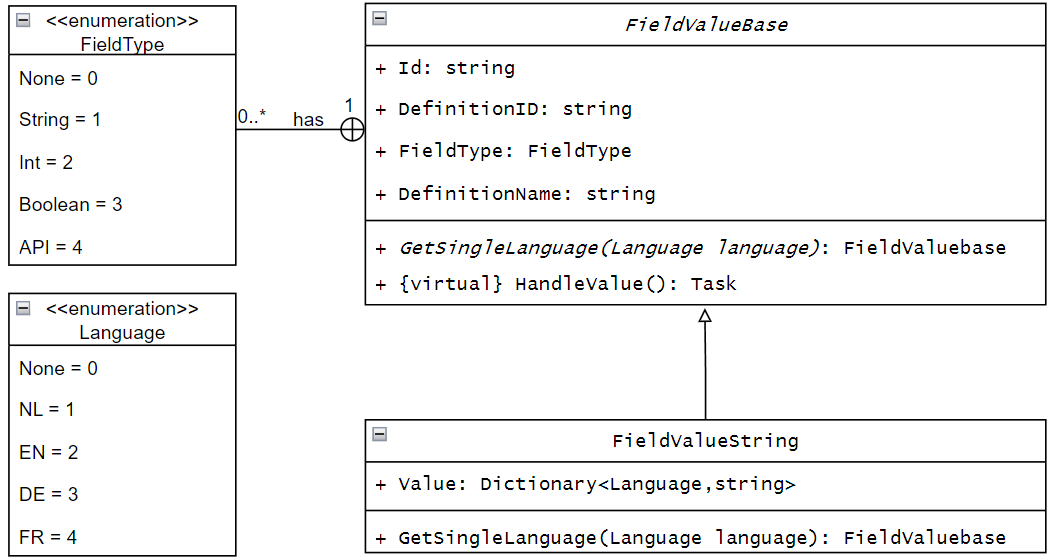
\includegraphics[scale=0.4]{FieldImplementation.png}
    \label{fig:ImplementatieFields}
\end{graphic}

\newpage

\whitespace
Een van de kenmerken van \textit{FieldValueString} is dat de data wordt opgeslagen in een dictionary met de taal als key.
% De huidige aanpak van het CMS voor meertaligheid houdt in dat een kopie van de originele site wordt gemaakt en vervolgens wordt vertaald.
Door vertalingen op te slaan in de \textit{fields}, kunnen vertalingen eenvoudig worden toegevoegd.
Dit resulteert in het onderhouden van slechts één site in plaats van een aparte site voor elke taal.

\whitespace
Het nadeel van een abstracte klasse als datatype gebruiken is dat de standaard C\# oplossing van \textit{Json Deserialisation} niet goed werkt.
Het probleem ligt in het interpreteren van de abstracte types naar de concrete implementaties.
Hierdoor kunnen controller endpoints niet de json data verwerken omdat er niet gedeserialiseerd mag worden van een abstracte klas.
Hierom wordt er gebruikgemaakt van een .NET 8 oplossing genaamd \textit{Model binders}.
Model binders zorgen ervoor dat controllers direct met het model kunnen werken in plaats van het HTTP request \parencite{ModelBinders}.
De geïmplementeerde versie van de model binder is te zien in figuur \ref{fig:Modelbinder}.
Verder zijn de mappers te zien die gebruikt worden in figuur \ref{fig:ModelbinderMappers}.

\whitespace
\begin{graphic}
    \captionsetup{type=figure}
    \caption{Item Modelbinder}
    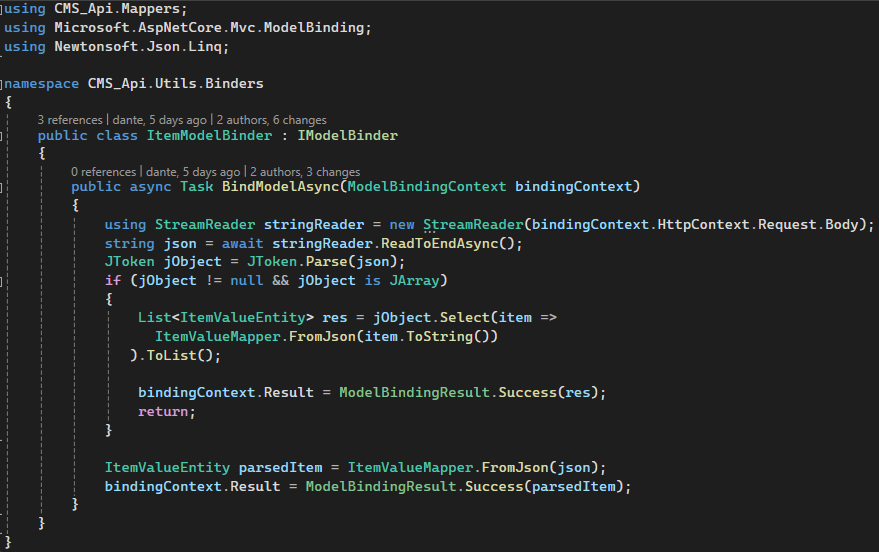
\includegraphics[scale=0.5]{ImplementatieModelBinder.png}
    \label{fig:Modelbinder}
\end{graphic}

\whitespace
\begin{graphic}
    \captionsetup{type=figure}
    \caption{Gebruikte mappers voor de modelbinder}
    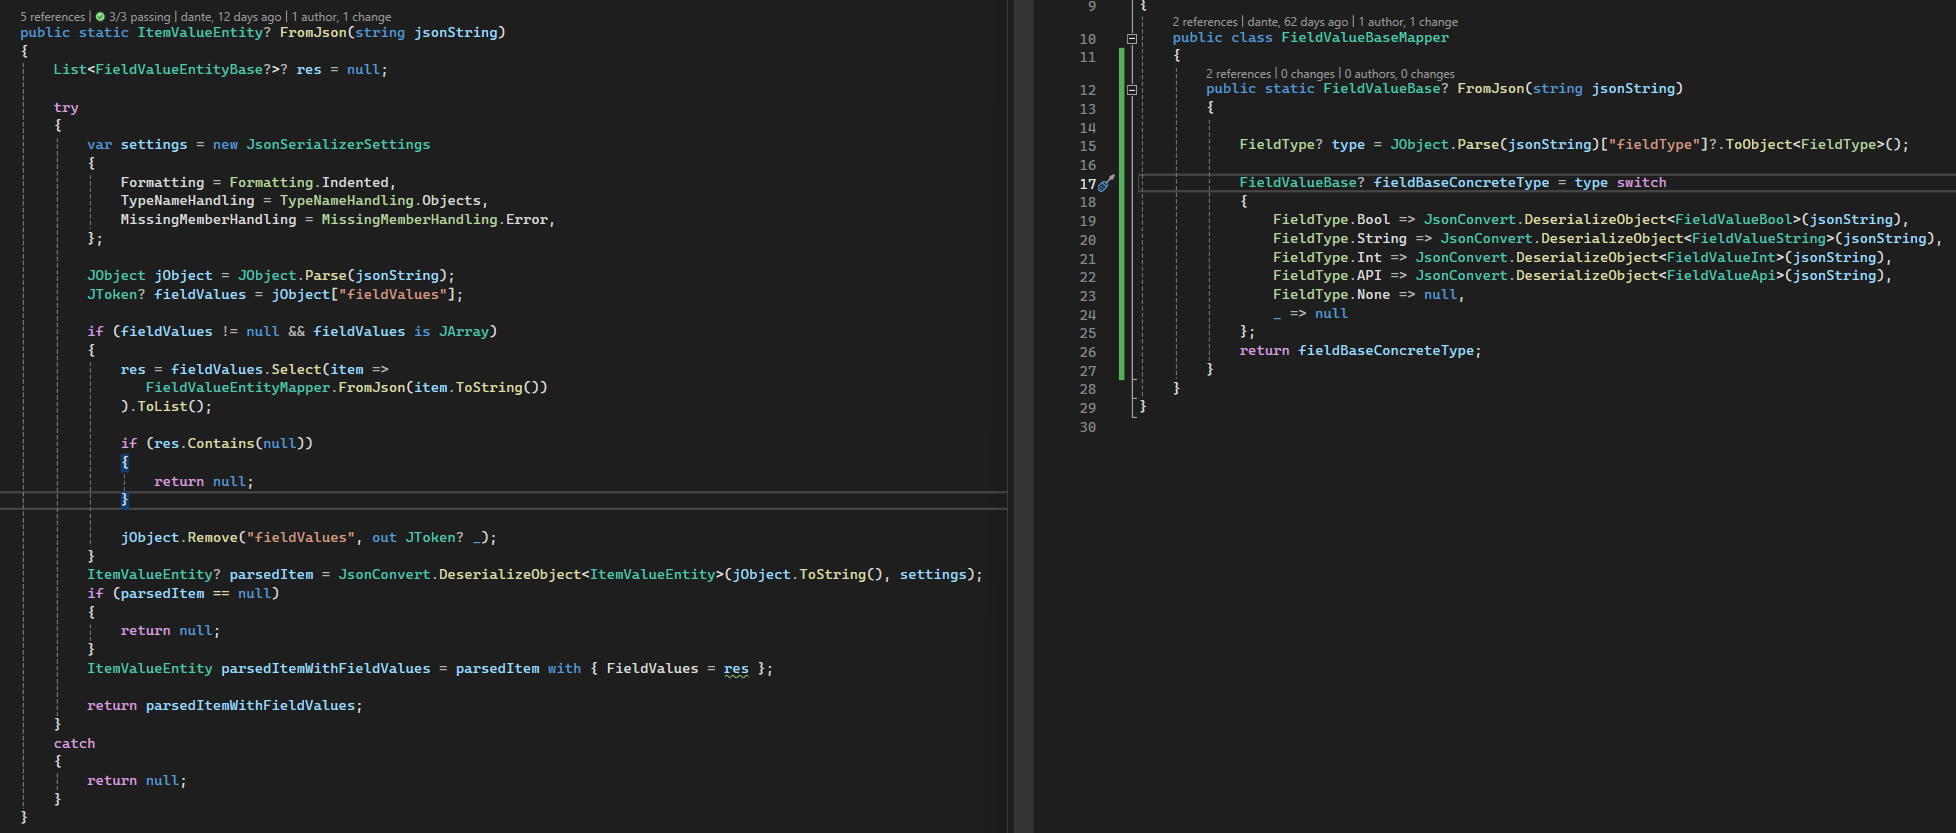
\includegraphics[scale=0.34]{implementatieModelBinderMappers.png}
    \label{fig:ModelbinderMappers}
\end{graphic}
